\documentclass[aspectratio=169,12pt]{beamer}
\usepackage[utf8]{inputenc}
\usepackage{amsmath, amssymb}
\usepackage{booktabs}
\usepackage{colortbl}
\usepackage{hyperref}
\usepackage{makecell}
\usepackage{ragged2e}
\usepackage{bytefield}
\usepackage{tikz}
\usetikzlibrary{arrows.meta, positioning, shapes.geometric, calc, tikzmark, shapes.misc, patterns, fit, circuits.logic.US, matrix, backgrounds}
\usepackage{circuitikz}
\usepackage{tcolorbox}
\usepackage{listings}
\usepackage{xcolor}
\usepackage{arydshln}
\usetheme{Madrid}

% Define blocksize length once globally
\newlength{\blocksize}
\setlength{\blocksize}{0.3cm}

% Define TikZ styles for cache diagrams
\tikzset{
    writeblock/.style={draw, thick, minimum width=\blocksize, minimum height=\blocksize, pattern=grid, pattern color=#1},
    writeblock/.default=blue
}

\newcommand{\addressbreakdown}[3]{%
    \begin{tikzpicture}[
        section/.style={draw, very thick, minimum height=0.6cm},
        bitnumber/.style={font=\tiny},
        sectionlabel/.style={font=\scriptsize},
        baseline=(current bounding box.center)
    ]
    % Calculate total bits and positions
    \pgfmathtruncatemacro{\totalbits}{#1 + #2 + #3}
    \pgfmathtruncatemacro{\tagstart}{\totalbits - 1}
    \pgfmathtruncatemacro{\tagend}{\totalbits - #1}
    \pgfmathtruncatemacro{\setstart}{\tagend - 1}
    \pgfmathtruncatemacro{\setend}{\tagend - #2}
    \pgfmathtruncatemacro{\offsetstart}{\setend - 1}
    \pgfmathtruncatemacro{\offsetend}{0}
    
    % Scale factor for width (adjust this to change overall size)
    \pgfmathsetmacro{\bitwidth}{0.17}
    
    % Starting position
    \pgfmathsetmacro{\xpos}{0}
    
    % Draw tag block
    \ifnum#1>0
        \pgfmathsetmacro{\tagwidth}{#1 * \bitwidth}
        \node[section, fill=blue!40, minimum width=\tagwidth cm] (tag) at (\xpos + \tagwidth/2, 0) {};
        \node[sectionlabel] at (tag.center) {tag};
        
        % Add bit numbers below
        \node[bitnumber] at ($(tag.south west) + (0mm,-1mm)$) {\tagstart};
        \node[bitnumber] at ($(tag.south east) + (-1mm,-1mm)$) {\tagend};
        
        \pgfmathsetmacro{\xpos}{\xpos + \tagwidth}
    \fi
    
    % Draw set block
    \ifnum#2>0
        \pgfmathsetmacro{\setwidth}{#2 * \bitwidth}
        \node[section, fill=green!40, minimum width=\setwidth cm] (set) at (\xpos + \setwidth/2, 0) {};
        % if num is smaller thean 2 rotate label
        \ifnum#2<3
            \node[sectionlabel, rotate=90] at (set.center) {set};
        \else
            \node[sectionlabel] at (set.center) {set};
        \fi

        % Add bit numbers below
        \node[bitnumber] at ($(set.south west) + (1mm,-1mm)$) {\setstart};
        \node[bitnumber] at ($(set.south east) + (-1mm,-1mm)$) {\setend};

        \pgfmathsetmacro{\xpos}{\xpos + \setwidth}
    \fi

    % Draw offset block
    \ifnum#3>0
        \pgfmathsetmacro{\offsetwidth}{#3 * \bitwidth}
        \node[section, fill=yellow!40, minimum width=\offsetwidth cm] (offset) at (\xpos + \offsetwidth/2, 0) {};
        \ifnum#3<3
            \node[sectionlabel, rotate=90, font=\tiny] at (offset.center) {offset};
        \else
            \node[sectionlabel] at (offset.center) {offset};
        \fi

        % Add bit numbers below - fix for when set bits = 0
        \ifnum#2>0
            \node[bitnumber] at ($(offset.south west) + (1mm,-1mm)$) {\offsetstart};
        \else
            % When no set bits, offset starts directly after tag
            \pgfmathtruncatemacro{\offsetstartalt}{\tagend - 1}
            \node[bitnumber] at ($(offset.south west) + (1mm,-1mm)$) {\offsetstartalt};
        \fi
        \node[bitnumber] at ($(offset.south east) + (0mm,-1mm)$) {\offsetend};
    \fi
    \end{tikzpicture}
}

% Alternative version with bit counts shown instead of labels
\newcommand{\addressbreakdownbits}[3]{%
    \begin{tikzpicture}[
        section/.style={draw, very thick, minimum height=0.8cm},
        bitnumber/.style={font=\tiny},
        bitcount/.style={font=\footnotesize},
        baseline=(current bounding box.center)
    ]
    % Calculate total bits and positions
    \pgfmathtruncatemacro{\totalbits}{#1 + #2 + #3}
    \pgfmathtruncatemacro{\tagstart}{\totalbits - 1}
    \pgfmathtruncatemacro{\tagend}{\totalbits - #1}
    \pgfmathtruncatemacro{\setstart}{\tagend - 1}
    \pgfmathtruncatemacro{\setend}{\tagend - #2}
    \pgfmathtruncatemacro{\offsetstart}{\setend - 1}
    \pgfmathtruncatemacro{\offsetend}{0}
    
    % Scale factor for width
    \pgfmathsetmacro{\bitwidth}{0.15}
    
    % Starting position
    \pgfmathsetmacro{\xpos}{0}
    
    % Draw tag block
    \ifnum#1>0
        \pgfmathsetmacro{\tagwidth}{#1 * \bitwidth}
        \node[section, fill=blue!40, minimum width=\tagwidth cm] (tag) at (\xpos + \tagwidth/2, 0) {};
        \node[bitcount] at (tag.center) {#1};
        
        % Add bit range below
        \node[bitnumber, below=2pt] at (tag.south) {\tagstart:\tagend};
        
        \pgfmathsetmacro{\xpos}{\xpos + \tagwidth}
    \fi
    
    % Draw set block
    \ifnum#2>0
        \pgfmathsetmacro{\setwidth}{#2 * \bitwidth}
        \node[section, fill=green!40, minimum width=\setwidth cm] (set) at (\xpos + \setwidth/2, 0) {};
        \node[bitcount] at (set.center) {#2};

        % Add bit range below
        \node[bitnumber, below=2pt] at (set.south) {\setstart:\setend};

        \pgfmathsetmacro{\xpos}{\xpos + \setwidth}
    \fi

    % Draw offset block
    \ifnum#3>0
        \pgfmathsetmacro{\offsetwidth}{#3 * \bitwidth}
        \node[section, fill=yellow!40, minimum width=\offsetwidth cm] (offset) at (\xpos + \offsetwidth/2, 0) {};
        \node[bitcount] at (offset.center) {#3};

        % Add bit range below - fix for when set bits = 0
        \ifnum#2>0
            \node[bitnumber, below=2pt] at (offset.south) {\offsetstart:\offsetend};
        \else
            % When no set bits, offset range is directly after tag
            \pgfmathtruncatemacro{\offsetstartalt}{\tagend - 1}
            \node[bitnumber, below=2pt] at (offset.south) {\offsetstartalt:\offsetend};
        \fi
    \fi

    % Add labels above
    \ifnum#1>0
        \node[font=\footnotesize, above=2pt] at (tag.north) {Tag};
    \fi
    \ifnum#2>0
        \node[font=\footnotesize, above=2pt] at (set.north) {Set};
    \fi
    \ifnum#3>0
        \node[font=\footnotesize, above=2pt] at (offset.north) {Offset};
    \fi
    \end{tikzpicture}
}

\title{Cache Memory I}
\author{Computer Architecture 234267}
\date{2025, Recitation \#3}

\begin{document}

\frame{\titlepage}

\begin{frame}{Outline}
\tableofcontents
\end{frame}

\section{Introduction}
\begin{frame}{The Problem}
\begin{itemize}
    \item Memory access speed is slow relative to processor performance (up to 1000x slower)
    \item The larger the memory, the slower the access
    \item Processor performance suffers significantly if we need to wait many clock cycles for each memory read
\end{itemize}
\end{frame}

\begin{frame}{The Solution}
\begin{center}
\textbf{Cache Memory}
\end{center}
\begin{itemize}
    \item Maintain a partial copy of memory "close" to the processor
    \item Access time is significantly shorter
    \item Exploits locality principles in programs
\end{itemize}
\end{frame}

\section{Locality Principles}
\begin{frame}{Why Does Cache Work?}
\begin{block}{Temporal Locality}
\begin{itemize}
    \item If we access an object, we're likely to access it again soon
    \item We spend 90\% of time in 10\% of code (loops)
    \item Certain variables are updated repeatedly
\end{itemize}
\end{block}

\begin{block}{Spatial Locality}
\begin{itemize}
    \item If we access an object, we're likely to access nearby objects
    \item Code segments: next instruction is likely needed
    \item Data: array elements are accessed sequentially
\end{itemize}
\end{block}

\textbf{Amdahl's Law Reminder:} Optimize what happens most of the time!
\end{frame}

\section{Cache Terminology}
\begin{frame}{Basic Terminology}
\begin{itemize}
    \item \textbf{Hit:} Data appears at the memory level
    \item \textbf{Miss:} Data doesn't appear at memory level, must fetch from lower level
    \item \textbf{Hit Rate:} Percentage of hits out of total memory accesses
    \item \textbf{Miss Rate:} $1 - \text{Hit Rate}$
    \item \textbf{Block:} Main memory is divided into blocks of several bytes. When copying a byte to cache, we copy the entire block
\end{itemize}
\end{frame}

\section{Cache Organizations}
\begin{frame}{Fully Associative Organization}
\begin{columns}
\column{0.5\textwidth}
\begin{itemize}
    \item Any block can map to any cache line
    \item Address divided into:
    \begin{itemize}
        \item Tag (block number)
        \item Offset (position within block)
    \end{itemize}
    \item Parallel comparison with all tags
\end{itemize}

\column{0.5\textwidth}
\begin{tcolorbox}[colback=gray!10]
\textbf{Address Fields:}\\
\begin{center}
    \addressbreakdown{27}{0}{5}
\end{center}
\end{tcolorbox}

\textbf{Advantage:} High hit rate\\
\textbf{Disadvantage:} Expensive parallel comparison
\end{columns}
\end{frame}

\begin{frame}{Fully Associative Cache - Structure}
\centering
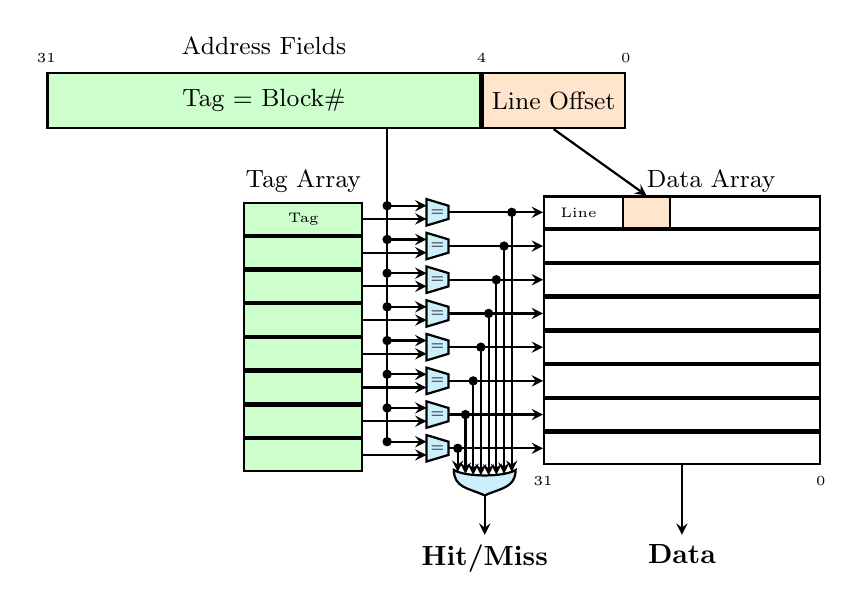
\begin{tikzpicture}[
    tagbox/.style={draw, thick, minimum width=1.5cm, minimum height=0.4cm, fill=green!20},
    databox/.style={draw, thick, minimum width=3.5cm, minimum height=0.4cm, fill=white},
    offsetbox/.style={draw, thick, minimum width=0.6cm, minimum height=0.4cm, fill=orange!20},
    label/.style={font=\small},
    biglabel/.style={font=\bfseries},
    data_connector/.style={circle, fill, inner sep=1.2pt},
    node distance=0cm
]

% Address breakdown at top
\node[draw, thick, fill=green!20, minimum width=5.5cm, minimum height=0.7cm, font=\small] (tag_field) {Tag = Block\#};
\node[label, font=\small, above=1mm of tag_field] (addr_title) {Address Fields};
\node[draw, thick, fill=orange!20, minimum width=1.2cm, minimum height=0.7cm, anchor=west, font=\small] (offset_field) at (tag_field.east) {Line Offset};
\node[label, font=\tiny, above] at (tag_field.north west) {31};
\node[label, font=\tiny, above] at (offset_field.west |- tag_field.north) {4};
\node[label, font=\tiny, above] at (offset_field.north east) {0};

% Labels for columns
\node[label, below=0.4cm of tag_field.south, xshift=0.5cm] (tag_array_label) {Tag Array};
\node[label, below=0.4cm of offset_field.south, xshift=2cm] (data_array_label) {Data Array};

% Create arrays using loops
\foreach \i in {0,...,7} {
    % Tag array - adjacent boxes (no space)
    \ifnum\i=0
        \node[tagbox, below=0cm of tag_array_label] (tag\i) {};
        \node[label, font=\tiny] at (tag\i.center) {Tag};
    \else
        \pgfmathtruncatemacro{\prev}{\i-1}
        \node[tagbox, below=0cm of tag\prev] (tag\i) {};
    \fi

    % Comparators using muxdemux - anchored at lpin 2 relative to tag
    \node[muxdemux, muxdemux def={Lh=0.6, Rh=0.3, NL=2, NB=1, w=0.5},
          external pins width=0, fill=cyan!20, anchor=lpin 2] (comp\i) at ([xshift=0.8cm]tag\i.east) {};
    % Add "=" inside comparator
    \node[font=\fontsize{4}{4}\selectfont] at (comp\i.center) {=};

    % Data array
    \node[databox, right=1.2cm of comp\i] (data\i) {};
}

\node[label, font=\tiny] at (data0.west) [anchor=west, xshift=1mm] {Line};
% Orange box only on first line
\node[offsetbox, anchor=west] at ([xshift=1cm]data0.west) (thedata) {};

% Tag input vertical line
\coordinate (tag_input_top) at ([xshift=-0.5cm]comp3.west);

% Connect tag input to all comparators
\foreach \i in {0,...,7} {
    \draw[->, >=stealth, thick] ([xshift=3mm]tag_field.south -| tag1.east) -- ([xshift=3mm]tag\i.east |- comp\i.lpin 1) node[data_connector] {}  -- (comp\i.lpin 1);
}

\draw[->, >=stealth, thick] (offset_field.south) -- (thedata.north);

% Connect arrays using loops
\foreach \i in {0,...,7} {
    % Tag to comparator (other input)
    \draw[->, >=stealth, thick] (tag\i.east) -- (comp\i.lpin 2);
    % Comparator to data
    \draw[->, >=stealth, thick] (comp\i.rpin 1) -- (data\i.west);
}

% OR gate for hit/miss
\node[or port, number inputs=8, anchor=north, external pins width=0, fill=cyan!20,
      xscale=0.7, yscale=0.3, rotate=-90, below right=0.5cm and 0.6cm of comp7.south, anchor=out] (or_gate) {};

% Connect comparators to OR gate
\foreach \i in {0,...,7} {
    \draw[->, >=stealth, thick] (comp\i.rpin 1) -- (comp\i.rpin 1 -| or_gate.bin \the\numexpr\i+1\relax) node[data_connector] {} -- (or_gate.bin \the\numexpr\i+1\relax);
}

% Hit/Miss output
\node[label, below=0.5cm of or_gate.bout, font=\bfseries] (hit_miss) {Hit/Miss};
\draw[->, >=stealth, thick] (or_gate.bout) -- (hit_miss.north);

% Data output
\node[label, font=\bfseries, anchor=north] (data_out) at (data7.south |- hit_miss.north east) {Data};
\draw[->, >=stealth, thick] (data7.south) -- (data_out.north);

% Bit labels at bottom
\node[label, font=\tiny] at ([yshift=-2mm]data7.south west) {31};
\node[label, font=\tiny] at ([yshift=-2mm]data7.south east) {0};

\end{tikzpicture}
\end{frame}

\begin{frame}{Direct Mapping Organization}
\begin{columns}
\column{0.5\textwidth}
\begin{itemize}
    \item Each block maps to exactly one cache location
    \item Address divided into:
    \begin{itemize}
        \item Tag (identifier)
        \item Set\# (cache location)
        \item Offset (position within block)
    \end{itemize}
    \item Simple indexing - no search needed
\end{itemize}

\column{0.5\textwidth}
\begin{tcolorbox}[colback=gray!10]
\textbf{Address Fields:}\\
\begin{center}
    \addressbreakdown{24}{3}{5}
\end{center}
\end{tcolorbox}

\textbf{Advantage:} Simple and cheap\\
\textbf{Disadvantage:} Higher miss rate due to conflicts
\end{columns}
\end{frame}

\begin{frame}
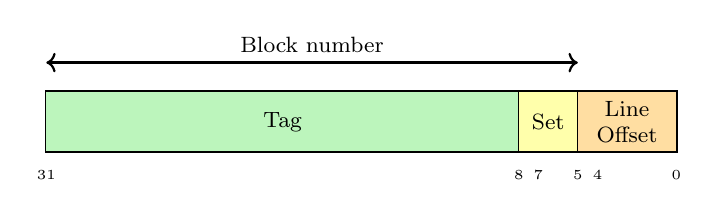
\begin{tikzpicture}[scale=0.25, font=\footnotesize]
  % Define constants
  \def\boxheight{3}
  
  % Define colors for different fields
  \definecolor{fieldgreen}{RGB}{144, 238, 144}
  \definecolor{fieldorange}{RGB}{255, 200, 100}
  \definecolor{fieldyellow}{RGB}{255, 255, 150}
  
  % Define key coordinates as base references
  \coordinate (origin) at (0,0);
  \coordinate (topright) at (32,\boxheight);
  
  % Draw outer border
  \draw[very thick] (origin) rectangle (topright);
  
  % Define field boundaries using coordinates
  % Working from MSB (31) to LSB (0), left to right
  \coordinate (b31) at (0,0);               % MSB position
  \coordinate (b8) at ($(b31) + (24,0)$);   % Tag is 24 bits wide (31-8)
  \coordinate (b5) at ($(b8) + (3,0)$);     % Set is 3 bits wide (7-5)
  \coordinate (b0) at ($(b5) + (5,0)$);     % Line Offset is 5 bits wide (4-0)
  
  % Tag field (31-8)
  \fill[fieldgreen!60] (b31) rectangle ($(b8) + (0,\boxheight)$);
  \draw[thick] (b8) -- ($(b8) + (0,\boxheight)$);
  \node at ($(b31)!0.5!(b8) + (0,\boxheight/2)$) {Tag};
  
  % Set field (7-5)
  \fill[fieldyellow!80] (b8) rectangle ($(b5) + (0,\boxheight)$);
  \draw[thick] (b5) -- ($(b5) + (0,\boxheight)$);
  \node at ($(b8)!0.5!(b5) + (0,\boxheight/2)$) {Set};
  
  % Line Offset field (4-0)
  \fill[fieldorange!60] (b5) rectangle ($(b0) + (0,\boxheight)$);
  \node[align=center] at ($(b5)!0.5!(b0) + (0,\boxheight/2)$) {Line\\Offset};
  
  % Add bit numbers below
  \node[below, font=\tiny] at ($(b31) + (0,-0.5)$) {31};
  \node[below, font=\tiny] at ($(b8) + (0,-0.5)$) {8};
  \node[below, font=\tiny] at ($(b8) + (1,-0.5)$) {7};
  \node[below, font=\tiny] at ($(b5) + (0,-0.5)$) {5};
  \node[below, font=\tiny] at ($(b5) + (1,-0.5)$) {4};
  \node[below, font=\tiny] at ($(b0) + (0,-0.5)$) {0};
  
  % Add "Block number" label with bracket above
  \draw[thick,<->] 
    ($(b31) + (0,\boxheight + 1.5)$) -- 
    ($(b5) + (0,\boxheight + 1.5)$)
    node[midway, above] {Block number};  

\end{tikzpicture}
\end{frame}

\begin{frame}{K-Way Set Associative Organization}
\begin{columns}
\column{0.5\textwidth}
\begin{itemize}
    \item Compromise between fully associative and direct mapped
    \item Cache divided into K ways
    \item Each block can map to K different locations (one per way)
    \item Most common: 2-way, 4-way, 8-way
\end{itemize}

\column{0.5\textwidth}
\begin{tcolorbox}[colback=gray!10]
\textbf{Example: 2-Way}\\
Each set has 2 possible locations\\
\vspace{0.3cm}
[Placeholder: 2-way cache diagram]
\end{tcolorbox}
\end{columns}
\end{frame}

\section{Replacement Policies}
\begin{frame}{Eviction Policies}
When cache is full and we need to bring in a new block, which block should be evicted?

\begin{enumerate}
    \item \textbf{LRU (Least Recently Used)}
    \begin{itemize}
        \item Evict the block that hasn't been used for the longest time
    \end{itemize}
    
    \item \textbf{LRM (Least Recently Modified)}
    \begin{itemize}
        \item Evict the block that hasn't been written to for the longest time
    \end{itemize}
    
    \item \textbf{Random}
    \begin{itemize}
        \item Completely random selection
    \end{itemize}
\end{enumerate}

Note: Direct mapped caches don't need replacement policy!
\end{frame}

\section{Write Policies}
\begin{frame}{Write Back Policy}
\begin{itemize}
    \item Write only to cache during write operation
    \item Update main memory only when block is evicted
    \item Requires a \textbf{dirty bit} per block to indicate if block was modified
    \item When evicting a block: update lower memory level only if dirty bit is set
\end{itemize}

\begin{center}
\begin{tcolorbox}[colback=blue!10, width=0.7\textwidth]
Write $\rightarrow$ L1 Cache (set dirty bit)\\
Eviction $\rightarrow$ If dirty, write to Memory
\end{tcolorbox}
\end{center}
\end{frame}

\begin{frame}{Write-Back Cache Operation}
\centering
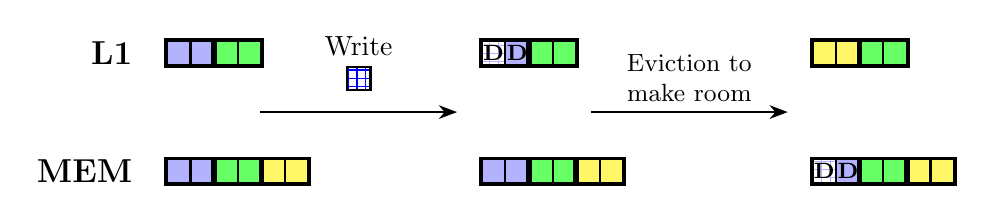
\begin{tikzpicture}[
    block/.style={draw, thick, minimum width=\blocksize, minimum height=\blocksize},
    label/.style={font=\bfseries\large},
    arrow/.style={->, >=Stealth, thick, font=\small},
    dirtymark/.style={font=\footnotesize\bfseries, black},
    group/.style={draw, very thick, inner sep=0pt},
    node distance=0cm and 0cm
]

% State 1: Initial
\node[label] (l1lbl) {L1};
\foreach \i/\col in {1/blue!30, 2/blue!30, 3/green!60, 4/green!60} {
    \node[block, fill=\col, right={\ifnum\i=1 0cm\else 0cm\fi} of l1lbl.east, 
          anchor=west, xshift={\i*\blocksize}] (s1_l1_\i) {};
}
% Group borders for State 1 L1
\node[group, fit=(s1_l1_1)(s1_l1_2)] {};
\node[group, fit=(s1_l1_3)(s1_l1_4)] {};

\node[label, below=1.5cm of l1lbl.east, anchor=east] (memlbl) {MEM};
\foreach \i/\col in {1/blue!30, 2/blue!30, 3/green!60, 4/green!60, 5/yellow!60, 6/yellow!60} {
    \node[block, fill=\col, right=0cm of memlbl.east,
          anchor=west, xshift={\i*\blocksize}] (s1_mem_\i) {};
}
% Group borders for State 1 MEM
\node[group, fit=(s1_mem_1)(s1_mem_2)] {};
\node[group, fit=(s1_mem_3)(s1_mem_4)] {};
\node[group, fit=(s1_mem_5)(s1_mem_6)] {};

% coordinate between L1 and MEM
\coordinate (between) at ($(l1lbl.east)!0.5!(memlbl.east)$);

% Arrow 1 with "Write" label
\draw[arrow] ([xshift=1.5cm]between) -- ++(2.5,0)
  node[midway, above] (arrow1) {};
\node[writeblock=blue,
      above=of arrow1] (writeblock) {};
\node[above=of writeblock] (write) {Write};

% State 2: After Write - positioned relative to arrow1
\coordinate (s2start) at ([xshift=4cm]between);

% L1 cache with first block (both pieces) marked as dirty
\foreach \i/\col in {1/blue!30, 2/blue!30, 3/green!60, 4/green!60} {
    \ifnum\i=1
        \node[writeblock=\col, 
              right=0cm of s2start, anchor=west, xshift={\i*\blocksize}, 
              yshift=0.75cm] (s2_l1_\i) {};
        % Add dirty bit marker
        \node[dirtymark] at (s2_l1_\i) {D};
    \else
        \ifnum\i=2
            \node[block, fill=\col, right=0cm of s2start,
                  anchor=west, xshift={\i*\blocksize}, yshift=0.75cm] (s2_l1_\i) {};
            % Add dirty bit marker to second piece of the block
            \node[dirtymark] at (s2_l1_\i) {D};
        \else
            \node[block, fill=\col, right=0cm of s2start,
                  anchor=west, xshift={\i*\blocksize}, yshift=0.75cm] (s2_l1_\i) {};
        \fi
    \fi
}
% Group borders for State 2 L1
\node[group, fit=(s2_l1_1)(s2_l1_2)] {};
\node[group, fit=(s2_l1_3)(s2_l1_4)] {};

% MEM remains unchanged in State 2
\foreach \i/\col in {1/blue!30, 2/blue!30, 3/green!60, 4/green!60, 5/yellow!60, 6/yellow!60} {
    \node[block, fill=\col, right=0cm of s2start,
          anchor=west, xshift={\i*\blocksize}, yshift=-0.75cm] (s2_mem_\i) {};
}
% Group borders for State 2 MEM
\node[group, fit=(s2_mem_1)(s2_mem_2)] {};
\node[group, fit=(s2_mem_3)(s2_mem_4)] {};
\node[group, fit=(s2_mem_5)(s2_mem_6)] {};

% Arrow 2
\coordinate (between2) at ([xshift=4*\blocksize+3cm]between);
\draw[arrow] ([xshift=1.5cm]between2) -- ++(2.5,0) 
    node[midway, above, align=center] (arrow2) {Eviction to\\make room};

% State 3: Final - after eviction
\coordinate (s3start) at ([xshift=4cm]between2);

% L1 cache with yellow blocks (new data loaded)
\foreach \i/\col in {1/yellow!60, 2/yellow!60, 3/green!60, 4/green!60} {
    \node[block, fill=\col, right=0cm of s3start,
          anchor=west, xshift={\i*\blocksize}, yshift=0.75cm] (s3_l1_\i) {};
}
% Group borders for State 3 L1
\node[group, fit=(s3_l1_1)(s3_l1_2)] {};
\node[group, fit=(s3_l1_3)(s3_l1_4)] {};

% MEM with updated first block (both pieces written back from cache)
\foreach \i/\col in {1/blue!30, 2/blue!30, 3/green!60, 4/green!60, 5/yellow!60, 6/yellow!60} {
    \ifnum\i=1
        \node[writeblock=\col,
              right=0cm of s3start, anchor=west, xshift={\i*\blocksize}, 
              yshift=-0.75cm] (s3_mem_\i) {};
        % Add dirty bit marker to show it was written back
        \node[dirtymark] at (s3_mem_\i) {D};
    \else
        \ifnum\i=2
            \node[block, fill=\col, right=0cm of s3start,
                  anchor=west, xshift={\i*\blocksize}, yshift=-0.75cm] (s3_mem_\i) {};
            % Add dirty bit marker to second piece of the block
            \node[dirtymark] at (s3_mem_\i) {D};
        \else
            \node[block, fill=\col, right=0cm of s3start,
                  anchor=west, xshift={\i*\blocksize}, yshift=-0.75cm] (s3_mem_\i) {};
        \fi
    \fi
}
% Group borders for State 3 MEM
\node[group, fit=(s3_mem_1)(s3_mem_2)] {};
\node[group, fit=(s3_mem_3)(s3_mem_4)] {};
\node[group, fit=(s3_mem_5)(s3_mem_6)] {};

\end{tikzpicture}

\vspace{1cm}
\footnotesize
\textbf{Note:} Write-back policy delays writes to main memory until cache line eviction.\\
The entire cache block (2 bytes) is marked dirty when any part is modified.\\
(Fully associative cache with 2 bytes per block, dirty blocks marked with 'D')
\end{frame}

\begin{frame}{Write-Through Cache Operation}
\centering
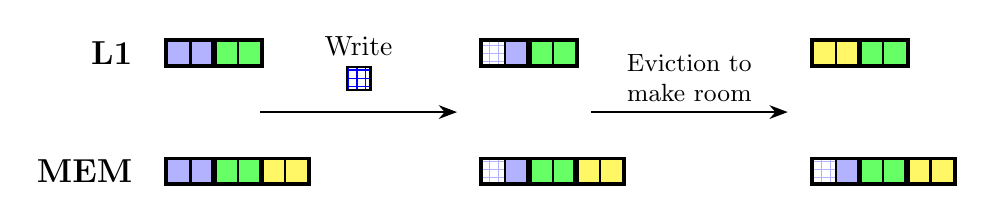
\begin{tikzpicture}[
    block/.style={draw, thick, minimum width=\blocksize, minimum height=\blocksize},
    label/.style={font=\bfseries\large},
    arrow/.style={->, >=Stealth, thick, font=\small},
    state/.style={inner sep=0pt},
    group/.style={draw, very thick, inner sep=0pt},
    node distance=0cm and 0cm
]
% Define colors for blocks
\def\initialL{blue!30, blue!30, green!60, green!60}
\def\initialM{blue!30, blue!30, green!60, green!60, yellow!60, yellow!60}

% State 1: Initial
\node[label] (l1lbl) {L1};
\foreach \i/\col in {1/blue!30, 2/blue!30, 3/green!60, 4/green!60} {
    \node[block, fill=\col, right={\ifnum\i=1 0cm\else 0cm\fi} of l1lbl.east, 
          anchor=west, xshift={\i*\blocksize}] (s1_l1_\i) {};
}
% Group borders for State 1 L1
\node[group, fit=(s1_l1_1)(s1_l1_2)] {};
\node[group, fit=(s1_l1_3)(s1_l1_4)] {};

\node[label, below=1.5cm of l1lbl.east, anchor=east] (memlbl) {MEM};
\foreach \i/\col in {1/blue!30, 2/blue!30, 3/green!60, 4/green!60, 5/yellow!60, 6/yellow!60} {
    \node[block, fill=\col, right=0cm of memlbl.east,
          anchor=west, xshift={\i*\blocksize}] (s1_mem_\i) {};
}
% Group borders for State 1 MEM
\node[group, fit=(s1_mem_1)(s1_mem_2)] {};
\node[group, fit=(s1_mem_3)(s1_mem_4)] {};
\node[group, fit=(s1_mem_5)(s1_mem_6)] {};

% coordinate between L1 and MEM
\coordinate (between) at ($(l1lbl.east)!0.5!(memlbl.east)$);

% Arrow 1
\draw[arrow] ([xshift=1.5cm]between) -- ++(2.5,0)
  node[midway, above] (arrow1) {};
\node[writeblock=blue, 
      above=of arrow1] (writeblock) {};
\node[above=of writeblock] (write) {Write};

% State 2: After Write - positioned relative to arrow1
\coordinate (s2start) at ([xshift=4cm]between);

\foreach \i/\col in {1/blue!30, 2/blue!30, 3/green!60, 4/green!60} {
    \ifnum\i=1
        \node[writeblock=\col, 
              right=0cm of s2start, anchor=west, xshift={\i*\blocksize}, 
              yshift=0.75cm] (s2_l1_\i) {};
    \else
        \node[block, fill=\col, right=0cm of s2start,
              anchor=west, xshift={\i*\blocksize}, yshift=0.75cm] (s2_l1_\i) {};
    \fi
}
% Group borders for State 2 L1
\node[group, fit=(s2_l1_1)(s2_l1_2)] {};
\node[group, fit=(s2_l1_3)(s2_l1_4)] {};

\foreach \i/\col in {1/blue!30, 2/blue!30, 3/green!60, 4/green!60, 5/yellow!60, 6/yellow!60} {
    \ifnum\i=1
        \node[writeblock=\col,
              right=0cm of s2start, anchor=west, xshift={\i*\blocksize}, 
              yshift=-0.75cm] (s2_mem_\i) {};
    \else
        \node[block, fill=\col, right=0cm of s2start,
              anchor=west, xshift={\i*\blocksize}, yshift=-0.75cm] (s2_mem_\i) {};
    \fi
}
% Group borders for State 2 MEM
\node[group, fit=(s2_mem_1)(s2_mem_2)] {};
\node[group, fit=(s2_mem_3)(s2_mem_4)] {};
\node[group, fit=(s2_mem_5)(s2_mem_6)] {};

% Arrow 2
\coordinate (between2) at ([xshift=4*\blocksize+3cm]between);
\draw[arrow] ([xshift=1.5cm]between2) -- ++(2.5,0) 
    node[midway, above, align=center] (arrow2) {Eviction to\\make room};

% State 3: Final - positioned relative to arrow2
\coordinate (s3start) at ([xshift=4cm]between2);

\foreach \i/\col in {1/yellow!60, 2/yellow!60, 3/green!60, 4/green!60} {
    \node[block, fill=\col, right=0cm of s3start,
          anchor=west, xshift={\i*\blocksize}, yshift=0.75cm] (s3_l1_\i) {};
}
% Group borders for State 3 L1
\node[group, fit=(s3_l1_1)(s3_l1_2)] {};
\node[group, fit=(s3_l1_3)(s3_l1_4)] {};

\foreach \i/\col in {1/blue!30, 2/blue!30, 3/green!60, 4/green!60, 5/yellow!60, 6/yellow!60} {
    \ifnum\i=1
        \node[writeblock=\col,
              right=0cm of s3start, anchor=west, xshift={\i*\blocksize}, 
              yshift=-0.75cm] (s3_mem_\i) {};
    \else
        \node[block, fill=\col, right=0cm of s3start,
              anchor=west, xshift={\i*\blocksize}, yshift=-0.75cm] (s3_mem_\i) {};
    \fi
}
% Group borders for State 3 MEM
\node[group, fit=(s3_mem_1)(s3_mem_2)] {};
\node[group, fit=(s3_mem_3)(s3_mem_4)] {};
\node[group, fit=(s3_mem_5)(s3_mem_6)] {};

\end{tikzpicture}

\vspace{1cm}
\footnotesize
\textbf{Note:} Write-through policy ensures data is written to both L1 cache and main memory simultaneously.\\
(Fully associative cache with 2 bytes per block)
\end{frame}




\begin{frame}{Write Through Policy}
\begin{itemize}
    \item Write to both cache AND main memory during write operation
    \item No need to update memory when block is evicted
    \item No dirty bit needed
    \item Simpler but more memory traffic
\end{itemize}

\begin{center}
\begin{tcolorbox}[colback=green!10, width=0.7\textwidth]
Write $\rightarrow$ L1 Cache + Memory (simultaneously)\\
Eviction $\rightarrow$ No memory update needed
\end{tcolorbox}
\end{center}
\end{frame}

\begin{frame}{Write Miss Policies}
What happens when we need to write to data not in cache?

\begin{block}{Write Allocate}
\begin{itemize}
    \item On write miss: fetch block from memory
    \item Allocate space in cache (may require eviction)
    \item Then perform the write
\end{itemize}
\end{block}

\begin{block}{No Write Allocate}
\begin{itemize}
    \item On write miss: write directly to memory
    \item Don't bring block to cache
    \item Simpler but may miss future locality
\end{itemize}
\end{block}
\end{frame}

\section{Types of Misses}
\begin{frame}{Three Types of Cache Misses}
\begin{enumerate}
    \item \textbf{Compulsory (Cold) Misses}
    \begin{itemize}
        \item Block has never been used before
        \item Unavoidable on first access
    \end{itemize}
    
    \item \textbf{Conflict Misses}
    \begin{itemize}
        \item Block was used but evicted due to mapping conflicts
        \item Another block took its place in the set
        \item Affected by associativity and mapping
    \end{itemize}
    
    \item \textbf{Capacity Misses}
    \begin{itemize}
        \item Block was used but evicted because cache is full
        \item Would occur even in fully associative cache
        \item Can only be reduced by increasing cache size
    \end{itemize}
\end{enumerate}
\end{frame}

\section{Detailed Examples}
\begin{frame}{Example 1: Cache Access Trace}
\textbf{Given:}
\begin{itemize}
    \item 2-way set associative cache, LRU replacement
    \item 4 bytes per block (line)
    \item Address format: %[Tag(29-5) | Set(4-2) | Offset(1-0)]
    \addressbreakdown{25}{3}{2}
    \item Sequence: 5, 7, 1, 4, 36, 8, 100, 6, 4, 12, 36, 12, 68, 5, 7
\end{itemize}

\textbf{Calculate:} Number of misses and final cache state
\end{frame}

\begin{frame}{Example 1: Solution Setup}
\textbf{Address Analysis:}
\begin{itemize}
    \item Block size = 4 bytes $\rightarrow$ 2 offset bits
    \item Addresses 0-3 $\rightarrow$ block 0, 4-7 $\rightarrow$ block 1, etc.
    \item Set = $\lfloor$Address / 4$\rfloor$ mod 4
\end{itemize}

\begin{center}
\begin{tabular}{|c|c|c|c|}
\hline
\textbf{Address} & \textbf{Block\#} & \textbf{Tag} & \textbf{Set} \\
\hline
5 & 1 & 0 & 1 \\
7 & 1 & 0 & 1 \\
1 & 0 & 0 & 0 \\
4 & 1 & 0 & 1 \\
36 & 9 & 1 & 1 \\
\hline
\end{tabular}
\end{center}
\end{frame}

\begin{frame}{Example 1: Trace Table}
\vspace{-0.5cm}
\begin{center}
\footnotesize
\begin{tabular}{|c|c:c|c|c|c|c|l|}
\hline
& \textbf{Addr} & \textcolor{blue}{\textbf{Tag}} \textcolor{green!70!black}{\textbf{Set}} \textcolor{orange}{\textbf{Off}} & \textbf{Tag} & \textbf{Set} & \textbf{H/M} & \textbf{\shortstack{Way/\\LRU}} & \textbf{Explanation} \\
\hline
1 & 5 & \textcolor{blue}{00}\textcolor{green!70!black}{001}\textcolor{orange}{01} & 0 & 1 & M & 0/1 & First access to set 1 \\
2 & 7 & \textcolor{blue}{00}\textcolor{green!70!black}{001}\textcolor{orange}{11} & 0 & 1 & H & 0/1 & Same block as addr 5 (4-7) \\
3 & 1 & \textcolor{blue}{00}\textcolor{green!70!black}{000}\textcolor{orange}{01} & 0 & 0 & M & 0/1 & First access to set 0 \\
4 & 4 & \textcolor{blue}{00}\textcolor{green!70!black}{001}\textcolor{orange}{00} & 0 & 1 & H & 0/1 & Already loaded (1) \\
5 & 36 & \textcolor{blue}{01}\textcolor{green!70!black}{001}\textcolor{orange}{00} & 1 & 1 & M & 1/0 & Different tag, set=1 (1), way=1 \\
6 & 8 & \textcolor{blue}{00}\textcolor{green!70!black}{010}\textcolor{orange}{00} & 0 & 2 & M & 0/1 & First access to set 2 \\
7 & 100 & \textcolor{blue}{11}\textcolor{green!70!black}{001}\textcolor{orange}{00} & 3 & 1 & M & 0/1 & Evict way 0 (LRU), set=1 \\
8 & 6 & \textcolor{blue}{00}\textcolor{green!70!black}{001}\textcolor{orange}{10} & 0 & 1 & M & 1/0 & Block 4-7 evicted (7), use way 0 (LRU) \\
9 & 4 & \textcolor{blue}{00}\textcolor{green!70!black}{001}\textcolor{orange}{00} & 0 & 1 & H & 1/0 & Loaded again (8) \\
10 & 12 & \textcolor{blue}{00}\textcolor{green!70!black}{011}\textcolor{orange}{00} & 0 & 3 & M & 0/1 & First access to set 3 \\
11 & 36 & \textcolor{blue}{01}\textcolor{green!70!black}{001}\textcolor{orange}{00} & 1 & 1 & M & 0/1 & Evict way 0 (LRU), set=1 \\
12 & 12 & \textcolor{blue}{00}\textcolor{green!70!black}{011}\textcolor{orange}{00} & 0 & 3 & H & 0/1 & Already loaded (10) \\
13 & 68 & \textcolor{blue}{10}\textcolor{green!70!black}{001}\textcolor{orange}{00} & 2 & 1 & M & 1/0 & Evict way 1 (LRU), set=1 \\
14 & 5 & \textcolor{blue}{00}\textcolor{green!70!black}{001}\textcolor{orange}{01} & 0 & 1 & M & 0/1 & Block evicted (8,13), use way 1 (LRU) \\
15 & 7 & \textcolor{blue}{00}\textcolor{green!70!black}{001}\textcolor{orange}{11} & 0 & 1 & H & 0/1 & Loaded again (14) \\
\hline
\end{tabular}
\end{center}
\end{frame}

\begin{frame}{Example 1: Final Results}
\textbf{Total Misses:} 11 out of 15 accesses

\textbf{Final Cache State:}
\begin{center}
\begin{tabular}{|c|c|c|}
\hline
\textbf{Set} & \textbf{Way 0} & \textbf{Way 1} \\
\hline
0 & Block 0 (tag 0) & Empty \\
1 & Block 1 (tag 0) & Block 17 (tag 2) \\
2 & Block 2 (tag 0) & Empty \\
3 & Block 3 (tag 0) & Empty \\
\hline
\end{tabular}
\end{center}

\textbf{Miss Types:} All are compulsory misses (each block accessed only once)
\end{frame}

\begin{frame}[fragile]{Example 2: Array Initialization}
\begin{columns}
\column{0.5\textwidth}
\begin{lstlisting}[language=C, basicstyle=\footnotesize\ttfamily, frame=single, backgroundcolor=\color{gray!10}]
int array[1024];
for (int i=0; i<1024; i++)
    array[i] = 0;
\end{lstlisting}

\textbf{Assumptions:}
\begin{itemize}
    \item i and array pointer in registers
    \item int = 4 bytes, aligned
    \item Array aligned to cache line
\end{itemize}

\column{0.5\textwidth}
\textbf{Cache specs:}
\begin{itemize}
    \item 1KB data cache
    \item 4-way set associative
    \item 16-byte blocks
    \item Write through
    \item Write allocate
    \item Random replacement
\end{itemize}
\end{columns}
\end{frame}

\begin{frame}{Example 2: Cache Directory Size}
\textbf{Question:} How many bits in the cache directory?

\textbf{Solution:}
\begin{itemize}
    \item Cache size: 1KB = 1024 bytes
    \item Block size: 16 bytes $\rightarrow$ 4 offset bits
    \item Number of blocks: $\frac{1024}{16} = 64$ blocks
    \item 4-way associative $\rightarrow$ 16 sets $\rightarrow$ 4 set bits
    \item Tag bits: 32 - 4 (offset) - 4 (set) = 24 bits
    \item Per line: 24 (tag) + 1 (valid) = 25 bits
    \item No dirty bit (write-through), No LRU bits (random)
\end{itemize}

\addressbreakdown{24}{4}{4}

\textbf{Total:} $25 \times 4 \times 16 = 1600$ bits
\end{frame}

\begin{frame}{Example 2: Number of Misses}
\textbf{Question:} Maximum number of misses during execution?

\textbf{Solution:}
\begin{itemize}
    \item Array size: $1024 \text{ints} \times 4 \text{bytes} = 4096 \text{bytes}$
    \item Block size: 16 bytes (4 ints per block)
    \item Total blocks needed: $\frac{4096}{16} = 256$ blocks
    \item Each block loaded once (compulsory miss)
    \item 4 ints per block $\rightarrow$ 3 hits after each miss
\end{itemize}


\textbf{Result:} 
\begin{itemize}
    \item 256 misses total
    \item Miss rate = $\frac{256}{1024} = 0.25 = 25\%$
    \item All are compulsory misses
\end{itemize}
\end{frame}

\begin{frame}{Example 2: Effect of Alignment}
\textbf{Question:} What if array is not aligned?

\textbf{Answer:}
\begin{itemize}
    \item If array starts at non-aligned address
    \item Array might span 257 blocks instead of 256
    \item First block: partial use
    \item Last block: partial use
    \item Maximum misses: 257 (one extra)
\end{itemize}

\begin{center}
\begin{tcolorbox}[colback=red!10, width=0.8\textwidth]
Alignment matters for cache performance!
\end{tcolorbox}
\end{center}
\end{frame}

\begin{frame}{Example 2: No Write Allocate}
\textbf{Question:} How many blocks transferred if using no-write-allocate?

Given: Variable i at address 0x00000100

\textbf{Solution:}
\begin{itemize}
    \item In the loop: only writing to array elements
    \item Only reading: variable i (for loop condition)
    \item With no-write-allocate:
    \begin{itemize}
        \item Writes go directly to memory
        \item Only i's block fetched to cache
    \end{itemize}
    \item Address 0x00000100 is aligned
\end{itemize}

\textbf{Result:} Only 1 block transferred to cache
\end{frame}

\begin{frame}{Example 2: Locality Principles}
\textbf{Question:} Which locality principle is demonstrated in this code?
\pause

\textbf{Reminder - Two Types of Locality:}
\begin{itemize}
    \item \textbf{Temporal:} If we access an object, we're likely to access it again soon
    \item \textbf{Spatial:} If we access an object, we're likely to access nearby objects
\end{itemize}
\pause

\textbf{Answer:} \textbf{Spatial Locality}
\begin{itemize}
    \item Array stored contiguously in memory
    \item When we miss on one element, we fetch entire block
    \item Next 3 elements are hits (same block)
    \item Spatial locality saves 3 misses per block
\end{itemize}
\pause

\textbf{NOT Temporal Locality:}
\begin{itemize}
    \item Each array element accessed only once
    \item No reuse of data
    \item But variable i shows temporal locality (accessed 1024 times)
\end{itemize}
\end{frame}

\section{Advanced Topics}
\begin{frame}{LRU Implementation for 4-Way Cache}
\textbf{Method 1: Full List (8 bits per set)}
\begin{itemize}
    \item Maintain linked list of 4 nodes (one per way)
    \item Store order of usage
    \item 2 bits per way $\times$ 4 ways = 8 bits
    \item Update list on every access
\end{itemize}

\textbf{Example states:}
\begin{center}
\begin{tabular}{|l|c|c|c|c|}
\hline
Initial: & Way0(00) & Way1(01) & Way2(10) & Way3(11) \\
Hit Way1: & Way1(01) & Way0(00) & Way2(10) & Way3(11) \\
Hit Way2: & Way2(10) & Way1(01) & Way0(00) & Way3(11) \\
\hline
\multicolumn{2}{|l}{MRU} & & & LRU \\
\hline
\end{tabular}
\end{center}
\end{frame}

\begin{frame}{LRU Implementation - Optimized}
\textbf{Method 2: Partial List (6 bits per set)}
\begin{itemize}
    \item Store only 3 most recent ways
    \item 4th way is implicitly LRU
    \item 2 bits $\times$ 3 = 6 bits per set
\end{itemize}

\textbf{Method 3: Optimal Encoding (5 bits per set)}
\begin{itemize}
    \item Number of possible orderings: $4! = 24$
    \item Need $\lceil \log_2(24) \rceil = 5$ bits
    \item Most space-efficient
    \item But complex encoding/decoding logic
\end{itemize}
\end{frame}

\begin{frame}{Segment-Based Cache Design}
\textbf{Problem:} Physical memory divided into 4 segments:
\begin{itemize}
    \item A0, B0, A1, B1 (256MB each)
    \item Requirement: Max 50\% cache for A segments, 50\% for B segments
\end{itemize}

\textbf{Solution:} Modified mapping function
\begin{itemize}
    \item Use MSB-2 bit to distinguish A (0) from B (1)
    \item Map sets 0--3 to A segments only
    \item Map sets 4--7 to B segments only
\end{itemize}

Original: [Tag | Set | Offset]\\
Modified: [Tag with segment bit | Modified Set | Offset]
\end{frame}

\begin{frame}{Cache Performance Metrics}
\textbf{Important Formulas:}
\begin{itemize}
    \item \textbf{Average Memory Access Time (AMAT):}
    $$AMAT = Hit\_Time + Miss\_Rate \times Miss\_Penalty$$
    
    \item \textbf{Cache Size:}
    $$Size = \#Sets \times \#Ways \times Block\_Size$$
    
    \item \textbf{Directory Size:}
    $$Dir\_Size = \#Sets \times \#Ways \times (Tag\_Bits + Status\_Bits)$$
    
    \item \textbf{Set Calculation:}
    $$Set = \lfloor Address / Block\_Size \rfloor \mod \#Sets$$
\end{itemize}
\end{frame}

\section{Example}
\begin{frame}{Example: Cache Access Pattern}
\begin{columns}
\column{0.5\textwidth}
\textbf{Given:}
\begin{itemize}
    \item 2-way set associative cache
    \item 4 bytes per block
    \item LRU replacement
    \item Address sequence (decimal):\\
    5, 7, 1, 4, 36, 8, 100, 6, 4, 12, 36, 12, 68, 5, 7
\end{itemize}

\column{0.5\textwidth}
\textbf{Address Format:}
\begin{tcolorbox}[colback=gray!10]
[Tag | Set | Offset]\\
29-5 | 4-2 | 1-0
\end{tcolorbox}

\textbf{Task:} Count hits and misses
\end{columns}
\end{frame}

\begin{frame}[fragile]{Example: Array Initialization}
\begin{columns}
\column{0.5\textwidth}
\begin{lstlisting}[language=C, basicstyle=\footnotesize\ttfamily, frame=single, backgroundcolor=\color{gray!10}]
int array[1024];
for (int i=0; i<1024; i++)
    array[i] = 0;
\end{lstlisting}

\textbf{Cache specs:}
\begin{itemize}
    \item 1KB data cache
    \item 4-way set associative
    \item 16-byte blocks
    \item Write through, write allocate
\end{itemize}

\column{0.5\textwidth}
\textbf{Analysis:}
\begin{itemize}
    \item Array size: 4KB (1024 $\times$ 4 bytes)
    \item Cache can hold: 64 blocks
    \item Array needs: 256 blocks
    \item Miss rate: 25\% (1 miss per 4 ints)
    \item Demonstrates spatial locality
\end{itemize}
\end{columns}
\end{frame}

\section{LRU Implementation}
\begin{frame}{LRU Implementation Strategies}
\textbf{For 4-way set associative cache:}

\begin{enumerate}
    \item \textbf{Full ordering (8 bits per set)}
    \begin{itemize}
        \item Maintain complete order of all 4 ways
        \item 2 bits per way $\times$ 4 ways = 8 bits
    \end{itemize}
    
    \item \textbf{Partial ordering (6 bits per set)}
    \begin{itemize}
        \item Track only 3 most recent ways
        \item Implicit LRU for 4th way
    \end{itemize}
    
    \item \textbf{Optimal encoding (5 bits per set)}
    \begin{itemize}
        \item 4! = 24 possible orderings
        \item Need $\lceil \log_2(24) \rceil = 5$ bits
    \end{itemize}
\end{enumerate}
\end{frame}


\tikzset{
    % Style definitions
    tagbox/.style={rectangle, draw, fill=green!30, minimum width=2cm, minimum height=0.6cm, font=\footnotesize},
    setbox/.style={rectangle, draw, fill=cyan!30, minimum width=1.5cm, minimum height=0.6cm, font=\footnotesize},
    offsetbox/.style={rectangle, draw, fill=orange!30, minimum width=2cm, minimum height=0.6cm, font=\footnotesize},
    cellstyle/.style={rectangle, draw, minimum width=1.2cm, minimum height=0.35cm, 
                     text depth=0.1cm, text height=0.2cm, font=\tiny},
    tagcell/.style={cellstyle, fill=green!20},
    titlecell/.style={cellstyle, font=\tiny},
    decoder/.style={muxdemux, muxdemux def={Lh=1, Rh=4, NB=0, NL=1, NR=4, w=0.8, square pins=0}, 
                   draw, fill=green!30, font=\tiny},
    % Comparator as downward-pointing pentagon
    comparator/.style={regular polygon, regular polygon sides=5, draw, fill=green!30, 
                      minimum width=1cm, minimum height=1cm, rotate=180},
    % MUX as wider trapezoid
    muxshape/.style={trapezium, trapezium angle=60, draw, minimum width=1.5cm, minimum height=0.8cm},
    arrow/.style={->, >=stealth, thick},
    dasharrow/.style={dashed, ->, >=stealth},
    % OR gate with custom sizing (rotated 90 degrees counter-clockwise)
    orgatestyle/.style={or gate US, draw, logic gate inputs=nn, anchor=center, 
                       minimum width=1cm, minimum height=0.8cm, rotate=90},
    % Junction dot style
    junction/.style={circle, fill=black, inner sep=0pt, minimum size=3pt}
}

\begin{frame}[fragile]{Cache Architecture}
\begin{center}
\begin{tikzpicture}[scale=0.8, transform shape]

% Address bits at top
\node[tagbox] (tag) {Tag};
\node[setbox, right=0pt of tag] (set) {Set};
\node[offsetbox, right=0pt of set] (offset) {Line Offset};

% Bit labels
\node[above=1mm of tag.west, anchor=south] {\footnotesize 31};
\node[above=1mm of tag.east, anchor=south] {\footnotesize 6};
\node[above=1mm of set.east, anchor=south] {\footnotesize 5\,4};
\node[above=1mm of offset.east, anchor=south] {\footnotesize 0};

% Define base positions for ways
\coordinate (way0base) at ($(set.south) + (-2.5,-2.5)$);
\coordinate (way1base) at ($(set.south) + (2.5,-2.5)$);

% Way 0 decoder (demux)
\node[decoder] at (way0base) (decoder0) {DEMUX};
\node[left=3mm of decoder0, font=\small] {Set\#};

% Way 0 Tag array matrix
\matrix[matrix of nodes, nodes={tagcell}, 
        column sep=-\pgflinewidth, row sep=-\pgflinewidth,
        right=8mm of decoder0.east, anchor=west, font=\tiny] (tag0) {
    |[titlecell]| Tag \\
    $\ldots$ \\
    $\vdots$ \\
    $\ldots$ \\
};

% Way 0 Data array - positioned relative to tag0
\matrix[matrix of nodes, nodes={cellstyle}, 
        column sep=-\pgflinewidth, row sep=-\pgflinewidth, font=\tiny] 
        at ($(tag0.east) + (0.8,0)$) (data0) {
    |[titlecell]| Data \\
    $\ldots$ \\
    $\vdots$ \\
    $\ldots$ \\
};

% Way 0 comparator - positioned relative to tag0
\node[comparator] at ($(tag0.south) + (0,-0.8)$) (comp0) {$=$};

% Way 0 label
\node[above=5mm of $(tag0.north)!0.5!(data0.north)$] (way0label) {\textbf{Way 0}};

% Way 1 decoder (demux)
\node[decoder] at (way1base) (decoder1) {DEMUX};
\node[left=3mm of decoder1, font=\small] {Set\#};

% Way 1 Tag array matrix
\matrix[matrix of nodes, nodes={tagcell}, 
        column sep=-\pgflinewidth, row sep=-\pgflinewidth,
        right=8mm of decoder1.east, anchor=west, font=\tiny] (tag1) {
    |[titlecell]| Tag \\
    \\
    $\vdots$ \\
    \\
};

% Way 1 Data array - positioned relative to tag1
\matrix[matrix of nodes, nodes={cellstyle}, 
        column sep=-\pgflinewidth, row sep=-\pgflinewidth, font=\tiny] 
        at ($(tag1.east) + (0.8,0)$) (data1) {
    |[titlecell]| Data \\
    \\
    $\vdots$ \\
    \\
};

% Way 1 comparator - positioned relative to tag1
\node[comparator] at ($(tag1.south) + (0,-0.8)$) (comp1) {$=$};

% Way 1 label
\node[above=5mm of $(tag1.north)!0.5!(data1.north)$] (way1label) {\textbf{Way 1}};

% Background for ways
\begin{pgfonlayer}{background}
    \node[fit=(way0label)(decoder0)(tag0)(data0)(comp0), 
          fill=gray!10, draw=gray!30, dashed, rounded corners, 
          inner sep=3mm] (way0bg) {};
    \node[fit=(way1label)(decoder1)(tag1)(data1)(comp1), 
          fill=gray!10, draw=gray!30, dashed, rounded corners, 
          inner sep=3mm] (way1bg) {};
\end{pgfonlayer}

% OR gate - positioned between comparators
\node[orgatestyle] at ($(comp0)!0.5!(comp1) + (0,-1.5)$) (orgate) {};

% MUX - positioned relative to data arrays
\node[muxshape] at ($(data0.south)!0.5!(data1.south) + (0,-2)$) (mux) {\footnotesize MUX};
% Define MUX connection points
\coordinate (muxin0) at ([yshift=0.2cm]mux.west);
\coordinate (muxin1) at ([yshift=0.2cm]mux.east);
\coordinate (muxsel) at (mux.north);

% Output labels
\node[below=0.8cm of orgate] (hitmiss) {Hit/Miss};
\node[below=0.5cm of mux] (dataout) {Data Out};

% Arrows from address bits to decoders with junction
\draw[arrow] (set.south) -- ++(0,-0.5) coordinate (setjunction);
\node[junction] at (setjunction) {};
\draw[arrow] (setjunction) -| (decoder0.north);
\draw[arrow] (setjunction) -| (decoder1.north);

% Arrows from address tag to comparators with junction
\draw[arrow] (tag.south) -- ++(0,-0.8) coordinate (tagjunction);
\node[junction] at (tagjunction) {};
\draw[arrow] (tagjunction) -| ([xshift=-0.3cm]comp0.south);
\draw[arrow] (tagjunction) -| ([xshift=-0.3cm]comp1.south);

% Arrows from offset to data arrays with junction
\draw[arrow] (offset.south) -- ++(0,-0.7) coordinate (offsetjunction);
\node[junction] at (offsetjunction) {};
\draw[arrow] (offsetjunction) -| ([yshift=0.3cm]data0.north);
\draw[arrow] (offsetjunction) -| ([yshift=0.3cm]data1.north);

\foreach \i in {1,2,3,4} {
    \draw[arrow] (decoder0.brpin \i) -- ([yshift={-(\i-2)*0.35cm}]tag0.west);
    \draw[arrow] (decoder1.brpin \i) -- ([yshift={-(\i-2)*0.35cm}]tag1.west);
}

% Dashed lines from tag arrays to data arrays (each row)
\foreach \i in {1,2,3,4} {
    \draw[dasharrow] ([yshift={-(\i-1)*0.35cm}]tag0.east) -- ([yshift={-(\i-1)*0.35cm}]data0.west);
    \draw[dasharrow] ([yshift={-(\i-1)*0.35cm}]tag1.east) -- ([yshift={-(\i-1)*0.35cm}]data1.west);
}

% Selected line highlighting (example: line 2)
\draw[arrow, thick, orange] ([yshift=-0.35cm]tag0.east) -- ++(0.2,0) coordinate (sel0);
\draw[arrow, thick, orange] (sel0) -- ([yshift=-0.35cm]data0.west);
\draw[arrow, thick, orange] ([yshift=-0.35cm]tag1.east) -- ++(0.2,0) coordinate (sel1);
\draw[arrow, thick, orange] (sel1) -- ([yshift=-0.35cm]data1.west);

% Tag array output to comparator
\draw[arrow] (tag0.south) -- ([xshift=0.3cm]comp0.south);
\draw[arrow] (tag1.south) -- ([xshift=0.3cm]comp1.south);

% Data array to MUX connections
\draw[arrow] (data0.south) |- (muxin0);
\draw[arrow] (data1.south) |- (muxin1);

% Comparator outputs to OR gate
\draw[arrow] (comp0.north) |- (orgate.input 1);
\draw[arrow] (comp1.north) |- (orgate.input 2);

% OR gate to Hit/Miss
\draw[arrow] (orgate.output) -- (hitmiss.north);

% Comparator to MUX select
\draw[arrow] (comp1.north) -- ++(0,-0.3) -| (muxsel);

% MUX to data out
\draw[arrow] (mux.south) -- (dataout.north);

\end{tikzpicture}
\end{center}
\end{frame}



\begin{frame}{Write Through Policy}
\begin{itemize}
    \item Write to both cache AND main memory during write operation
    \item No need to update memory when block is evicted
    \item \alert{No dirty bit needed} (Why?)
    \item Simpler but more memory traffic
\end{itemize}

\begin{center}
\begin{tcolorbox}[colback=green!10, width=0.8\textwidth]
\begin{tabular}{c c c}
Write & $\rightarrow$ & L1 Cache \\
      & $\searrow$ & Memory (simultaneously)\\
& & \\
Eviction & $\rightarrow$ & No memory update needed
\end{tabular}
\end{tcolorbox}
\end{center}

\textbf{Note:} Valid bit still needed to indicate if cache line contains valid data
\end{frame}

\begin{frame}{Write Miss Policies: Write Allocate}
\textbf{Write Allocate:}
\begin{enumerate}
    \item On write miss: send request to fetch block from memory
    \item Before fetching: free appropriate location (based on set and replacement policy)
    \item Fetch block from lower level
    \item Perform the write to cache
\end{enumerate}

\begin{center}
\begin{tcolorbox}[colback=yellow!10, width=0.9\textwidth]
Write request, miss $\rightarrow$ Evict if needed $\rightarrow$ Fetch block $\rightarrow$ Write to cache
\end{tcolorbox}
\end{center}

Commonly used with \textbf{write-back} policy
\end{frame}

\begin{frame}{Write Miss Policies: No Write Allocate}
\textbf{No Write Allocate:}
\begin{itemize}
    \item On write miss: send write request directly to memory
    \item Don't fetch block to cache
    \item No eviction needed
    \item Simpler but may miss future locality
\end{itemize}

\begin{center}
\begin{tcolorbox}[colback=orange!10, width=0.7\textwidth]
Write request, miss $\rightarrow$ Write directly to memory\\
(Cache unchanged)
\end{tcolorbox}
\end{center}

Commonly used with \textbf{write-through} policy
\end{frame}

\section{Advanced Topics}
\begin{frame}{LRU Implementation for 4-Way Cache}
\textbf{Method 1: Full List (8 bits per set)}
\begin{itemize}
    \item Maintain linked list of 4 nodes (one per way)
    \item Store order of usage
    \item 2 bits per way $\times$ 4 ways = 8 bits
    \item Update list on every access
\end{itemize}

\textbf{Example states:}
\begin{center}
\begin{tabular}{|l|c|c|c|c|}
\hline
Initial: & Way0(00) & Way1(01) & Way2(10) & Way3(11) \\
Hit Way1: & Way1(01) & Way0(00) & Way2(10) & Way3(11) \\
Hit Way2: & Way2(10) & Way1(01) & Way0(00) & Way3(11) \\
\hline
\multicolumn{2}{|l}{MRU} & & & LRU \\
\hline
\end{tabular}
\end{center}
\end{frame}

\begin{frame}{LRU Implementation - Optimized}
\textbf{Method 2: Partial List (6 bits per set)}
\begin{itemize}
    \item Store only 3 most recent ways
    \item 4th way is implicitly LRU
    \item 2 bits × 3 = 6 bits per set
\end{itemize}

\textbf{Method 3: Optimal Encoding (5 bits per set)}
\begin{itemize}
    \item Number of possible orderings: 4! = 24
    \item Need $\lceil \log_2(24) \rceil = 5$ bits
    \item Most space-efficient
    \item But complex encoding/decoding logic
\end{itemize}
\end{frame}

\begin{frame}{Segment-Based Cache Design}
\textbf{Problem:} Physical memory divided into 4 segments:
\begin{itemize}
    \item A0, B0, A1, B1 (256MB each)
    \item Requirement: Max 50\% cache for A segments, 50\% for B segments
\end{itemize}

\textbf{Solution:} Modified mapping function
\begin{itemize}
    \item Use MSB-2 bit to distinguish A (0) from B (1)
    \item Map sets 0-3 to A segments only
    \item Map sets 4-7 to B segments only
\end{itemize}

Original: [Tag | Set | Offset]\\
Modified: [Tag with segment bit | Modified Set | Offset]
\end{frame}

\begin{frame}{Cache Performance Metrics}
\textbf{Important Formulas:}

\begin{itemize}
    \item \textbf{Average Memory Access Time (AMAT):}
    $$AMAT = Hit\_Time + Miss\_Rate \times Miss\_Penalty$$
    
    \item \textbf{Cache Size:}
    $$Size = \#Sets \times \#Ways \times Block\_Size$$
    
    \item \textbf{Directory Size:}
    $$Dir\_Size = \#Sets \times \#Ways \times (Tag\_Bits + Status\_Bits)$$
    
    \item \textbf{Set Calculation:}
    $$Set = \lfloor Address / Block\_Size \rfloor \mod \#Sets$$
\end{itemize}
\end{frame}

\begin{frame}{Advanced Example: Segment-Based Cache Design}
\textbf{Problem Setup:}
\begin{itemize}
    \item 2-way set associative cache deployed in a system
    \item Physical memory divided into 4 equal segments (256MB each):
    \begin{itemize}
        \item A0, B0, A1, B1 (in this order)
    \end{itemize}
    \item \textbf{Design Requirement:} No more than 50\% of cache should contain addresses from A segments OR B segments
    \item Must maintain 2-way associativity
\end{itemize}

\textbf{Question:} Propose a simple and efficient method to implement this requirement and explain its operation.
\end{frame}

\begin{frame}{Segment-Based Cache: Analysis}
\textbf{Step 1: Understanding Memory Segments}
\begin{itemize}
    \item Each segment is 256MB = $2^{28}$ bytes
    \item Total memory: 1GB = 4 segments
    \item Need 30 bits to address 1GB (ignoring upper 2 bits)
\end{itemize}
\pause

\textbf{Step 2: Segment Encoding in Address Bits}
\begin{center}
\begin{tabular}{|c|c|c|}
\hline
\textbf{Segment} & \textbf{Bits [29:28]} & \textbf{Address Range} \\
\hline
A0 & 00 & 0x00000000 - 0x0FFFFFFF \\
B0 & 01 & 0x10000000 - 0x1FFFFFFF \\
A1 & 10 & 0x20000000 - 0x2FFFFFFF \\
B1 & 11 & 0x30000000 - 0x3FFFFFFF \\
\hline
\end{tabular}
\end{center}
\pause

\textbf{Key Observation:}
\begin{itemize}
    \item Bit 28: distinguishes A (0) from B (1) segments
    \item This single bit can control cache partitioning!
\end{itemize}
\end{frame}

\begin{frame}{Segment-Based Cache: Solution}
\textbf{Design Goal:} Ensure max 50\% cache for A segments, 50\% for B segments

\pause
\textbf{Original Cache Mapping (8 sets example):}
\begin{itemize}
    \item Address format: \addressbreakdown{25}{3}{2}
    \item Any address can map to any set (0-7)
    \item Problem: A segments could occupy 100\% of cache!
\end{itemize}

\pause
\textbf{Solution: Modified Set Mapping}
\begin{itemize}
    \item Include segment bit (bit 28) in set calculation
    \item New set field: concatenate bit 28 with original set bits
    \item Result: Sets 0-3 for A segments, Sets 4-7 for B segments
    \item Modified address format:
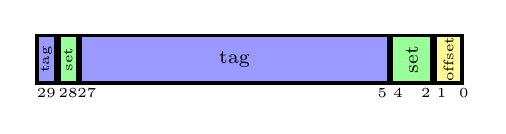
\begin{tikzpicture}[
    section/.style={draw, very thick, minimum height=0.6cm},
    bitnumber/.style={font=\tiny},
    sectionlabel/.style={font=\scriptsize},
    baseline=(current bounding box.center)
]
    % Tag section - bit 29
    \node[section, fill=blue!40, minimum width=0.17cm] (tag29) at (0,0) {};
    \node[sectionlabel, rotate=90, font=\tiny] at (tag29.center) {tag};
    \node[bitnumber] at ($(tag29.south) + (0mm,-1mm)$) {29};

    % Set section - bit 28 (segment bit)
    \node[section, fill=green!40, minimum width=0.17cm, anchor=west] (set28) at (tag29.east) {};
    \node[sectionlabel, rotate=90, font=\tiny] at (set28.center) {set};
    \node[bitnumber] at ($(set28.south) + (0mm,-1mm)$) {28};

    % Tag section - bits 27-5
    \node[section, fill=blue!40, minimum width=3.91cm, anchor=west] (tag275) at (set28.east) {};
    \node[sectionlabel] at (tag275.center) {tag};
    \node[bitnumber] at ($(tag275.south west) + (1mm,-1mm)$) {27};
    \node[bitnumber] at ($(tag275.south east) + (-1mm,-1mm)$) {5};

    % Set section - bits 4-2
    \node[section, fill=green!40, minimum width=0.51cm, anchor=west] (set42) at (tag275.east) {};
    \node[sectionlabel, rotate=90] at (set42.center) {set};
    \node[bitnumber] at ($(set42.south west) + (1mm,-1mm)$) {4};
    \node[bitnumber] at ($(set42.south east) + (-1mm,-1mm)$) {2};

    % Offset section - bits 1-0
    \node[section, fill=yellow!40, minimum width=0.34cm, anchor=west] (offset) at (set42.east) {};
    \node[sectionlabel, rotate=90, font=\tiny] at (offset.center) {offset};
    \node[bitnumber] at ($(offset.south west) + (1mm,-1mm)$) {1};
    \node[bitnumber] at ($(offset.south east) + (0mm,-1mm)$) {0};
\end{tikzpicture}
\end{itemize}
\end{frame}

\begin{frame}{Segment-Based Cache: Concrete Example}
\textbf{Example Addresses and Their Mapping:}

\begin{center}
\begin{tabular}{|c|c|c|c|}
\hline
\textbf{Address} & \textbf{Segment} & \textbf{Bit 28} & \textbf{Maps to Set} \\
\hline
\texttt{0x05000010} & A0 & 0 & 0-3 (A sets) \\
\texttt{0x12345678} & B0 & 0 & 4-7 (B sets) \\
\texttt{0x25000000} & A1 & 1 & 0-3 (A sets) \\
\texttt{0x3ABCDEF0} & B1 & 1 & 4-7 (B sets) \\
\hline
\end{tabular}
\end{center}

\pause
\vspace{0.5cm}
\textbf{Cache Organization Result:}
\begin{columns}
\column{0.5\textwidth}
\begin{center}
\textbf{Sets 0-3: A segments only}
\begin{itemize}
    \item Can cache data from A0 and A1
    \item Maximum 50\% of total cache
    \item 2-way associative within group
\end{itemize}
\end{center}

\column{0.5\textwidth}
\begin{center}
\textbf{Sets 4-7: B segments only}
\begin{itemize}
    \item Can cache data from B0 and B1
    \item Maximum 50\% of total cache
    \item 2-way associative within group
\end{itemize}
\end{center}
\end{columns}

\begin{tcolorbox}[colback=green!10]
\textbf{Advantages:} Simple hardware, guaranteed 50/50 split, maintains associativity
\end{tcolorbox}
\end{frame}

\section{Summary}
\begin{frame}{Cache Design Trade-offs}
\begin{table}
\centering
\small
\begin{tabular}{lcc}
\toprule
\textbf{Design Choice} & \textbf{Advantage} & \textbf{Disadvantage} \\
\midrule
Fully Associative & High hit rate & Expensive hardware \\
Direct Mapped & Simple, cheap & Higher miss rate \\
Set Associative & Good compromise & Moderate complexity \\
\midrule
Write Back & Less memory traffic & Needs dirty bit, complexity \\
Write Through & Simple, consistent & More memory traffic \\
\midrule
Write Allocate & Good locality exploitation & Transfer overhead \\
No Write Allocate & Simple, less traffic & May miss reuse \\
\midrule
Large blocks & Better spatial locality & More transfer time \\
Small blocks & Less wasted transfer & Poor spatial locality \\
\bottomrule
\end{tabular}
\end{table}
\end{frame}

\begin{frame}{Key Takeaways}
\begin{itemize}
    \item Cache exploits temporal and spatial locality
    \item Set associativity provides good performance/cost trade-off
    \item Write policies affect memory traffic and complexity
    \item Different miss types require different optimizations:
    \begin{itemize}
        \item Compulsory: Larger blocks, prefetching
        \item Conflict: Increase associativity
        \item Capacity: Increase cache size
    \end{itemize}
    \item Implementation details matter:
    \begin{itemize}
        \item Alignment affects performance
        \item LRU can be optimized for space
        \item Directory overhead is significant
    \end{itemize}
    \item Real systems use multi-level hierarchies (L1, L2, L3)
\end{itemize}
\end{frame}

\end{document}